% !TEX TS-program = pdflatex
% !TEX encoding = UTF-8 Unicode

% This is a simple template for a LaTeX document using the "article" class.
% See "book", "report", "letter" for other types of document.

\documentclass[12pt,drafta4paper,oneside]{memoir} % use larger type; default would be 10pt

\usepackage[utf8]{inputenc} % set input encoding (not needed with XeLaTeX)
\usepackage[margin=2cm]{geometry}
\usepackage{xy}
\usepackage{amsmath, amsthm}
\usepackage{showkeys}
\usepackage{acronym}
\usepackage[marginclue]{fixme}
%\usepackage{natbib}
\usepackage{tabularx}
\usepackage{chngpage}
\usepackage{booktabs}
\usepackage{cite}
\usepackage{times}
\usepackage{graphicx}
\usepackage{ctable}
\usepackage{footnote}
\fxsetup{
    status=draft,
    author=,
    layout=marginclue,inline, % also try footnote or pdfnote
    theme=color
}
\definecolor{fxnote}{rgb}{0.8000,0.0000,0.0000}

\OnehalfSpacing
\setcounter{tocdepth}{3}

\usepackage{color}
\usepackage{listings}
\lstset{ %
language=C++,                % choose the language of the code
basicstyle=\ttfamily,       % the size of the fonts that are used for the code
numbers=left,                   % where to put the line-numbers
numberstyle=\footnotesize,      % the size of the fonts that are used for the line-numbers
stepnumber=1,                   % the step between two line-numbers. If it is 1 each line will be numbered
numbersep=5pt,                  % how far the line-numbers are from the code
backgroundcolor=\color{white},  % choose the background color. You must add \usepackage{color}
showspaces=false,               % show spaces adding particular underscores
showstringspaces=false,         % underline spaces within strings
showtabs=false,                 % show tabs within strings adding particular underscores
frame=single,           % adds a frame around the code
tabsize=2,          % sets default tabsize to 2 spaces
captionpos=b,           % sets the caption-position to bottom
breaklines=false,        % sets automatic line breaking
breakatwhitespace=false,    % sets if automatic breaks should only happen at whitespace
escapeinside={\%*}{*)}          % if you want to add a comment within your code
}

%%% END Article customizations

%%% The "real" document content comes below...

\title{VPR Assessment of a Novel Partitioning Algorithm}
\author{David Munro}
%\date{} % Activate to display a given date or no date (if empty),
         % otherwise the current date is printed

\begin{document}
\maketitle
\begin{abstract}
	Space based systems, etc, so we want "To implement the partitioning algorithm and assess the results using Versatile Place and Route (VPR) and MCNC benchmarks".
\end{abstract}
\chapter*{Acknowledgements}
Thanking various people

\newpage
\acrodef{VPR}[VPR]{Versatile Place and Route}
\acrodef{MCNC}[MCNC]{Microelectronics Centre of North Carolina}
\acrodef{BLE}[BLE]{Basic Logic Element}
\acrodef{CLB}[CLB]{Configurable Logic Block}
\acrodef{DFG}[DFG]{Directed Flow Graph}
\acrodef{SEU}[SEU]{Single Event Upset}
\acrodef{LUT}[LUT]{Look Up Table}
\acrodef{VTR}[VTR]{Verilog To Routing}
\acrodef{STL}[STL]{Standard Template Library}
\acrodef{FPGA}[FPGA]{Field Programmable Gate Array}
\acrodef{TMR}[TMR]{Triple Modular Redundancy}
\acrodef{BLIF}[BLIF]{Berkeley Logic Interchange Format}
\acrodef{ASIC}[ASIC]{Application Specific Integrated Circuit}
\acrodef{LAB}[LAB]{Logic Array Block}
\acrodef{IO}[I/O]{Input/Output}
\tableofcontents*
\chapter{Introduction}
\section{Overview}
•To implement the partitioning algorithm and assess the results using Versatile Place and Route (VPR) and MCNC (Microelectronics Centre of North Carolina) benchmarks.
•VPR used as it’s open source.

•What are we partitioning and why?
•FPGA’s are useful for space based applications due to low cost, wide availability, etc. [1].
•Downsides include increased susceptibility to radiation induced errors[1]. For Virtex 4 in geosynchronous orbit, predicted mean time between errors is only 1.4s[2].
•Use Triple Modular Redundancy (TMR) to detect errors.
\subsection{FPGA}
What is an FPGA?
--------------------------------------------------------------------------------
\acp{FPGA} are popular devices capable of implementing a wide variety of circuits. Unlike \ac{ASIC} circuits which must be specially designed and manufactured for an application---a lengthy and expensive process---\acp{FPGA} are a generic device which can be mass produced by manufacturers and then adapted for individual user's needs. Their flexibility, low cost, and faster development process make them popular for a number of applications.

An \ac{FPGA} consists of a grid of \acp{CLB} (sometimes called \acp{LAB}), generally containing flip flops and \acp{LUT}; a number of \ac{IO} blocks, allowing for inputs and outputs from the \ac{FPGA}; and routing channels containing the wires between blocks.
\fixme{TODO: Use own image. Wilton lecture notes have no license/copyright notice/etc attached, so don't know if this usage is actually allowed. Wouldn't come under Fair Use}
\begin{figure}
    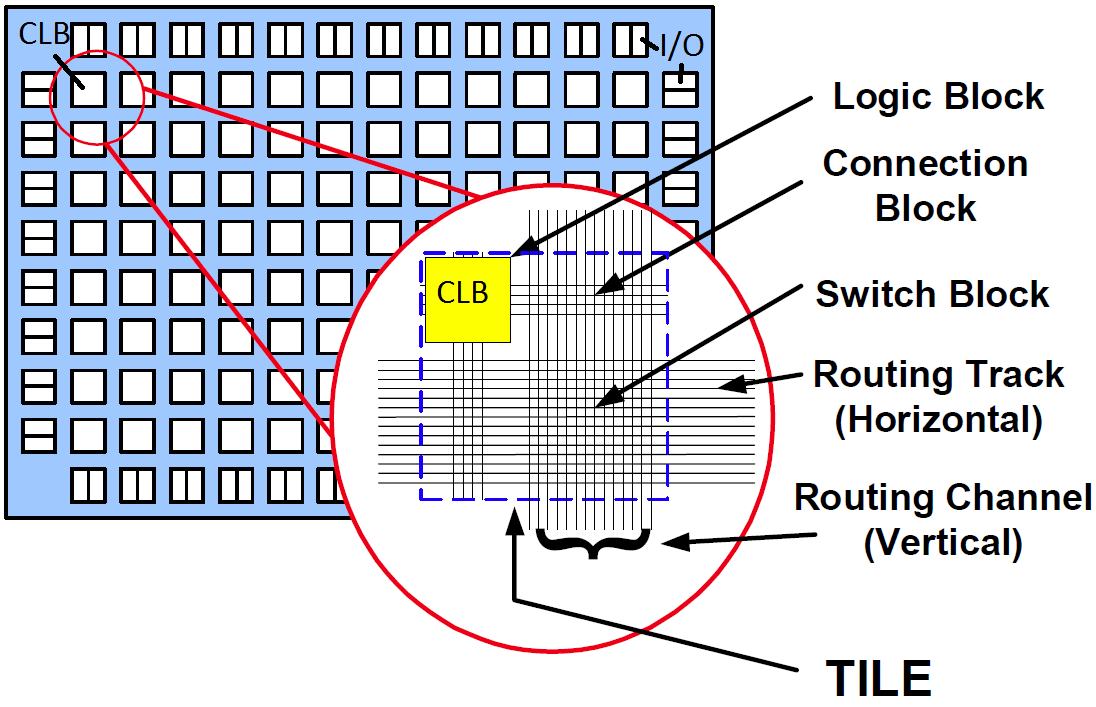
\includegraphics[width=\textwidth]{images/fpga-arch.png}
    \caption{FPGA Architecture\cite{WiltonLecture}}
    \label{FPGAArch}
\end{figure}
An n-input Look Up Table (written as n-LUT) can be programmed to represent any n-input boolean function, while latches allow for register transfer operations. A \ac{CLB} is made up of a number of smaller blocks, called \acp{BLE}, with each block containing the flips flops and \acp{LUT}. There is then programmable routing both within each \ac{CLB} and in between \acp{CLB}.


There are three main components to an \ac{FPGA}. \ac{IO} blocks, usually around the edge, allowing for input and output from the \ac{FPGA}, \acp{CLB} containing all the logic elements (\acp{LUT}, latches, etc), and the routing between everything.
The routing between everything consists of channels running horizontally and vertically with a number of wires. Programmable switches connect the wires to each other and to \acp{CLB} allowing for configurable paths between arbitrary components. A typical switch or connection block has a buffer storing the state, and a connection can be made or unmade by writing a new value to the buffer for that switch.
\acp{CLB} are a cluster of smaller blocks, called \acp{BLE}, with each \ac{BLE} containing the basic logic elements, typically a programmable \ac{LUT} for combinational logic, a latch for register operations and allowing sequential logic, and a \ac{mux} to switch between the two. As with the switches in routing, buffers store the values for the \ac{LUT}, whether the \ac{mux} is selecting the latch or \ac{LUT} output, and other switch states.

Programming an \ac{FPGA} involves loading in a bitstream which describes all the component values (i.e. contents of each buffer) for a circuit. A number of \acp{FPGA} also allow for run time programming, or reconfiguration of parts of a circuit, which involves loading the bitstream for just section of interest while the rest of the \ac{FPGA} keeps running.

There are four main technologies used to implement the reprogrammable buffers in \acp{FPGA}: \ac{SRAM}, which gives the highest density devices and includes the Virtex 5 family this thesis focuses on, however are volatile and must be reprogrammed every power up from an external configuration memory; (anti)fuse, which are only one time programmable; EPROM, \ac{EEPROM}, which are reprogrammable, non-volatile this not requiring an external configuration memory, however have a lower density than \ac{SRAM} \acp{FPGA}.

The reprogrammable buffers can be implemented using a storage technology of choice, however in practice there only three technologies which see common use:\fixme{TODO: reference} \ac{SRAM}, which gives the highest density devices and includes the Virtex 5 family this thesis focuses on, however are volatile and must be reprogrammed every power up from an external configuration memory; antifuse, which are only one time programmable; and \ac{EEPROM}, which are reprogrammable and non-volatile, thus not requiring an external configuration memory, however have a lower density than \ac{SRAM} \acp{FPGA}. \fixme{TODO: reference}

\subsubsection{Partial Reconfiguration}
Partial reconfiguration involves loading configuration information for part of a circuit during operation. Much like the complete configuration described above, which happens at power up, it involves writing a configuration bitstream to one of the available configuration ports, in this case also including the location to reconfigure. The configuration memory of recent Virtex devices is split into frames, and one can only reconfigure entire frames. As more frames are being reconfigured the larger the bitstream, and consequently the longer the time to reconfigure. The main configuration ports used are the external SelectMAP interface, or the internal \ac{ICAP}, each with a bandwidth of 400MB/s in all Virtex devices \fixme{TODO: reference: tc-draft}.


\subsection{Space Based Applications}
Space is quite different from a terrestrial environment, and one \acp{FPGA} have a number of advantages in due to their lower \ac{NRE} costs and flexibility. As \acp{FPGA} can be reconfigured during a mission, faulty/outdated designs can be replaced remotely. However, there is a significant downside. As systems go further into space, and are no longer protected by the earth's atmosphere\fixme{TODO: Check this}, they become increasingly likely to suffer from radiation induced errors, where ionising radiation intersecting with a component causes charge build up, potentially triggering incorrect operation\cite{SEEMechanism}. Of the potential effects, which range from unnoticeable to device destruction, this thesis is concerned with mitigating \acp{SEU}, where an incorrect signal is triggered, but the underlying hardware still operates correctly. \fixme{TODO: Add in table and diagram}. In an \ac{ASIC} \acp{SEU} are transient. While the erroneous pulse may cause run on effects, be latched, or otherwise affect the circuit in future, the component itself continues operating normally.
\acp{FPGA} on the other hand, are vulnerable to permanent configuration errors as well. When the charged particle impacts a buffer it can flip the state of the buffer changing the actual circuit. Unlike transient errors, these errors persist indefinitely. \fixme{TODO: images of this. Picture of transient, picture of permanent. Need to be a slideshow?}
Additionally for \ac{SRAM} devices, the off-chip configuration memory itself can be affected, so the next time the chip is reprogrammed (e.g. after power cycling), an incorrect circuit will be loaded.

(Anti)fuse devices, being non reprogrammable, are immune to these errors, however both \ac{SRAM} and \ac{EEPROM} based \acp{FPGA} are vulnerable \fixme{TODO: reference}.

\subsection{How we deal with FPGA downsides}
Clearly in order for \acp{FPGA} to be viable in space based systems the effects of \acp{SEU} must be mitigated. A number of technologies and techniques are available, each with their own advantages and disadvantages.
There are three main categories of \ac{SEU} hardening techniques\cite{HardeningTechniques}:
\begin{itemize}
    \item Charge dissipation, which aims to keep the effect of the radiation below the level where it would have an effect. This includes techniques such as increasing the drive current. These techniques typically require custom hardware (increasing costs) and usually increase power usage.
    \item Temporal Filtering, which aims to filter out transient \acp{SEU}, such as delay-and-vote\cite{HardeningTechniques}. These techniques often slow down operation and are ineffective against configuration errors.
    \item Spatial Redundancy, which uses multiple redundant circuits to detect errors, and be able to continue operating. Spatial redundancy techniques are split into those which provide hardware level redundancy, such as \ac{DICE}, with slightly increased area usage, increased power, and often increased component time, and those which provide design level redundancy, such as \ac{TMR}, which increase area and power usage significantly (see Table \ref{HardeningComparison}), however require no custom hardware and greatly improve the circuit's hardness. As the area is increased a common side effect is a decrease in maximum operating frequency, however unlike some temporal filtering options the actual component speed remains the same.
\end{itemize}
While hardened \acp{FPGA} are available, they typically lag well behind mainstream commercial offerings\cite{VFPGATMR}, thus solutions which can be implemented on typical \ac{FGPA} hardware are desirable. Additionally, there is very little point hardening an \ac{FPGA} and not its configuration buffers and memory which take up far more surface area\fixme{TODO: reference} and are thus even more vulnerable.
For these reasons \ac{TMR}, requiring no custom hardware and \ac{SEU} protection against both transient outputs, as well as to its configuration, is one of the more popular \ac{SEU} hardening techniques.

\begin{table}
    \begin{tabularx}{\textwidth}{X|XXXl}
   & POWER & SPEED & HARDNESS (e/b-d) & AREA ($\mbox{mm}^2$)\\
Std Low Power & Rise – 0.7 \mu W \newline Fall – 0.2 \mu W & Rise – 0.21 ns \newline Fall – 0.27 ns & 10E-8 \newline 1 node & 360\\
Increased IDRIVE & Rise – 1.0 \mu W \newline Fall – 0.2 \mu W & Rise – 0.16 ns \newline Fall – 0.15 ns & 2\times10E-9 \newline 1 node & 460\\
\ac{TMR} & Rise – 1.72 \mu W \newline Fall – 1.27 \mu W & Rise – 0.21 ns \newline Fall – 0.27 ns & 10E-11 \newline 2 node & 1200\\
DICE & Rise - 1.4\mu W \newline Fall - 1.1\mu  W & Rise - 0.96 ns \newline Fall - 0.97ns & 1.6\times10E-10 \newline 2 node & 520 \\
    \end{tabularx}
    \caption{Comparison of hardening techniques\cite{HardeningTechniques}}
    \label{HardeningComparison}
\end{table}

One additional technique specific to \ac{SRAM} based \acp{FPGA} relates to the protection of the off-chip configuration memory. As \ac{SRAM} is volatile and loads the state from off chip at power up, this external configuration memory must also be protected from \acp{SEU}. This can be accomplished by incorporating error detection and correction techniques in the RAM, something already in place on a number of mainstream \acp{FPGA} such as the Virtex-4 and 5\cite{


\section{Triple Modular Redundancy}
Triple Modular Redundancy is a commonly used method for creating fault tolerant systems in which a given circuit is implemented three times with independent components, with the outputs feeding into a voter circuit to determine the majority value. For any \ac{SEU} it will affect the output value of at most one circuit, so the majority vote is still correct. One can then incorporate partial reconfiguration in order to recover from detected errors, as described in \fixme{TODO: reference}. However, this only works when at most one \ac{SEU} occurs within the error detection and recovery time. Should \acp{SEU} occur in two of the three partitions then it can be impossible for the voter to determine the correct value. Therefore, we require the error detection and recovery time to be sufficiently small that the likelihood of multiple events occurring within that time period are negligible.
The error recovery time consists of the time to reconfigure the circuit, which is a function of the circuit area, and the resynchronisation time, which is a function of critical path and clock frequency, so it is required that our area and critical path length are small enough, and frequency large enough, that our error recovery time is within a user specified system availability threshold.
\begin{eqnarray*}
    \mbox{Error Recovery Time} &=& \mbox{Error Detection Time} + \mbox{Reconfiguration Time} + \mbox{Resynchronisation Time}\\
    \frac{1}{\mbox{Error Recovery Time}} &=& \mbox{System Availability}
\end{eqnarray*}
\begin{eqnarray*}
    \mbox{Error Detection Time} <= \frac{1}{\mbox{Clock Frequency}}\times\mbox{Pipeline Steps}
\end{eqnarray*}
\begin{eqnarray*}
    \mbox{Reconfiguration Time} &=& \frac{1}{\mbox{Reconfiguration Speed}}\times\mbox{Bitstream Size}\\
     &=& \fixme{TODO: Actual Values}\times\mbox{Partition Size in Slices}
\end{eqnarray*}
\begin{eqnarray*}
    \mbox{Resynchronisation Time} <= \frac{1}{\mbox{Clock Frequency}}\times\mbox{Pipeline Steps}
\end{eqnarray*}
Additionally, as each voter circuit adds some constant overhead, in terms of area, power usage and clock frequency slowdown, so it is desirable to have each partition as large as possible. This thesis is primarily concerned with implementing and assessing this form of \ac{TMR}, with a discussion of other \ac{TMR} methods and our reasons for not using them following.
\subsection{Prior Work, lit review, etc?}
Some lit review and prior work stuff.
-----------------------------------------------------------------------------------------
This thesis builds on the work of \fixme{TODO: reference} which details a partitioning algorithm that traverses a circuit represented as a \ac{DFG} in a breadth first manner, creating partitions that stay within our constraints.
Our goal is to create an algorithm which gives good performance, stays within a user specified system availability limit, doesn't require existing code to be rewritten, allows for both voting logic and reconfiguration logic to be added, can use industry standard \acp{FPGA}, and effectively protects the entire system from \acp{SEU}. There are a number of existing \ac{TMR} solutions, however none quite meet our requirements.
Our first requirement is that standard \ac{FPGA} hardware can be used, with our implementation specifically targeting Virtex 5 chips. Options with custom hardware such as \cite{VFPGATMR}, are often prohibitively expensive, and prevent us from using our existing boards.
Most manufacturer boards with inbuilt hardware, in addition to requiring custom hardware, typically only provide partial protection, e.g.\cite{Synplify}.
\cite{ftmr} requires existing code to be rewritten.
\cite{synplify} and \cite{tmrtool} don't seem to support staying within a system availability limit, nor for adding reconfiguration logic.
Other options look at using partial \ac{TMR} to reduce the associated overhead (\cite{partialTMR}), require custom hardware (\cite{VFPGATMR}), or otherwise don't meet our criteria.

\cite{FPGAReview},\cite{VTMR}

\section{CAD Design Flow}
Talking about the overall CAD design flow. ODIN -> ABC -> Partitioner -> VPR, etc.
\begin{figure}
    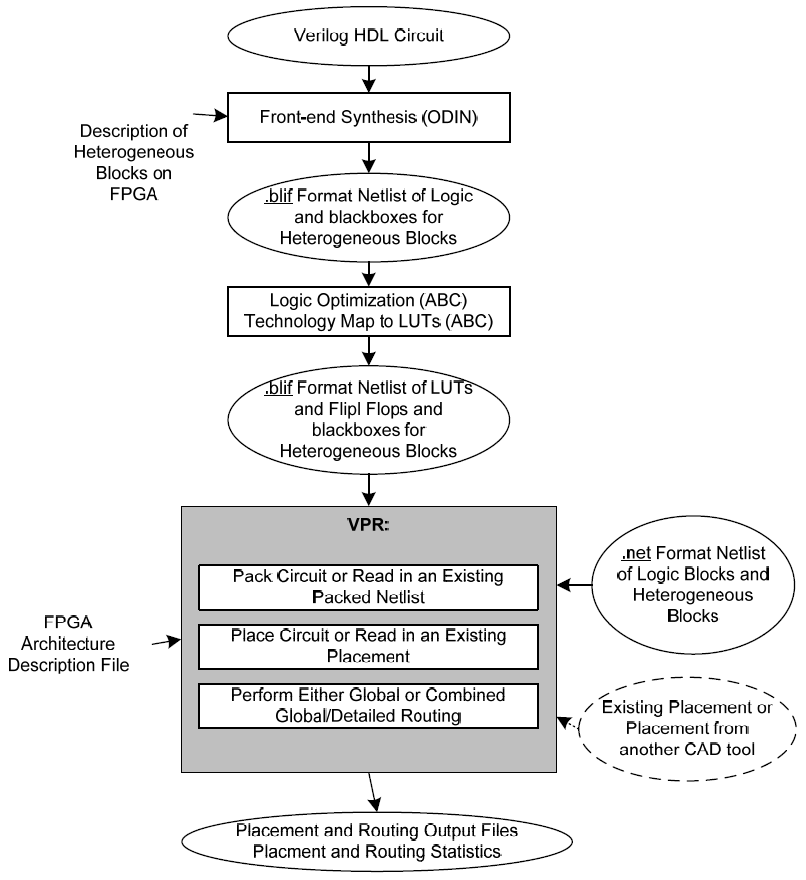
\includegraphics[width=\textwidth]{images/vpr-cad.png}
    \caption{Cad Design Flow. Sourced from TODO:}
    \label{CADFlow}
\end{figure}
\subsection{How VPR Works}
Default settings for VPR and what they all change, algorithms used, etc.

\chapter{Benchmarking}
\section{Overview}
We have a number of benchmark circuits (detailed in \ref{benchmarkList}) which we will be using to evaluate the performance of our partitioner and our \ac{TMR} scheme in general.
Additionally, we're looking for ways of estimating area usage and timing information from a \ac{BLIF} file or \ac{DFG}, without needing to actually place and route the partial circuit after each iteration, as we desire a partitioner with speed of the same order as the other steps in the \ac{CAD} flow.

To start with we make simple test circuits to compare to our benchmarks by triplicating each entire benchmark and adding in simple voter logic. As progress is made on the partitioner we can start collecting results from further partitioned circuits, however triplicating the entire circuit should be sufficient for approximations, provided $elements_{circuit} >> elements_{voter}$.

To make the test circuits we created a small Python script to, given an input circuit and input voter circuit, triplicate the circuit and add voting logic. It creates a hierarchical \ac{BLIF} file, that is, it contains nested subcircuits, which are then passed through \ac{SIS} to flatten it into a format \ac{VPR} can read.

\begin{table}
    \begin{tabular}{c|cccc}
     & \multicolumn{4}{c}{Number of:}\\
     Name & Inputs & Outputs & Latches & Combinational Logic Elements\\
        alu4 & 14 & 8 & 0 & 4574\\
        apex2 & 38 & 3 & 0 & 5637\\
        apex4 & 9 & 19 & 0 & 3805\\     
        bigkey & 229 & 197 & 672 & 5294\\
        clma & 62 & 82 & 99 & 25177\\
        des & 256 & 245 & 0 & 5018\\
        diffeq & 64 & 39 & 1131 & 4521\\
        dsip & 229 & 197 & 672 & 4283\\
        elliptic & 131 & 114 & 3366 & 10920\\
        ex1010 & 10 & 10 & 0 & 13804\\
        ex5p & 8 & 63 & 0 & 3255\\
        frisc & 20 & 116 & 2658 & 10733\\
        misex3 & 14 & 14 & 0 & 4205\\
        pdc & 16 & 40 & 0 & 13765\\
        s298     & 4 & 6 & 24 & 5796\\
        s38417   & 29 & 106 & 4389 & 18232\\
        s38584.1 & 38 & 304 & 3780 & 18835\\
        seq      & 41 & 35 & 0 & 5285\\
        spla     & 16 & 46 & 0 & 11116\\
        tseng    & 52 & 122 & 1155 & 3260
    \end{tabular}
    \caption{Benchmark circuits used}
    \label{benchmarkList}
\end{table}


\section{Why VPR}
\ac{VPR} is an open source packer, placer, and router commonly used for research. We chose \ac{VPR} as, largely due to it being open source and popular, it is well documented, uses easy to read file formats, and is easy to modify if necessary. Additionally, all of the algorithms used to place and route are available and well described in literature.

\subsection{Architecture File}
\begin{figure}
    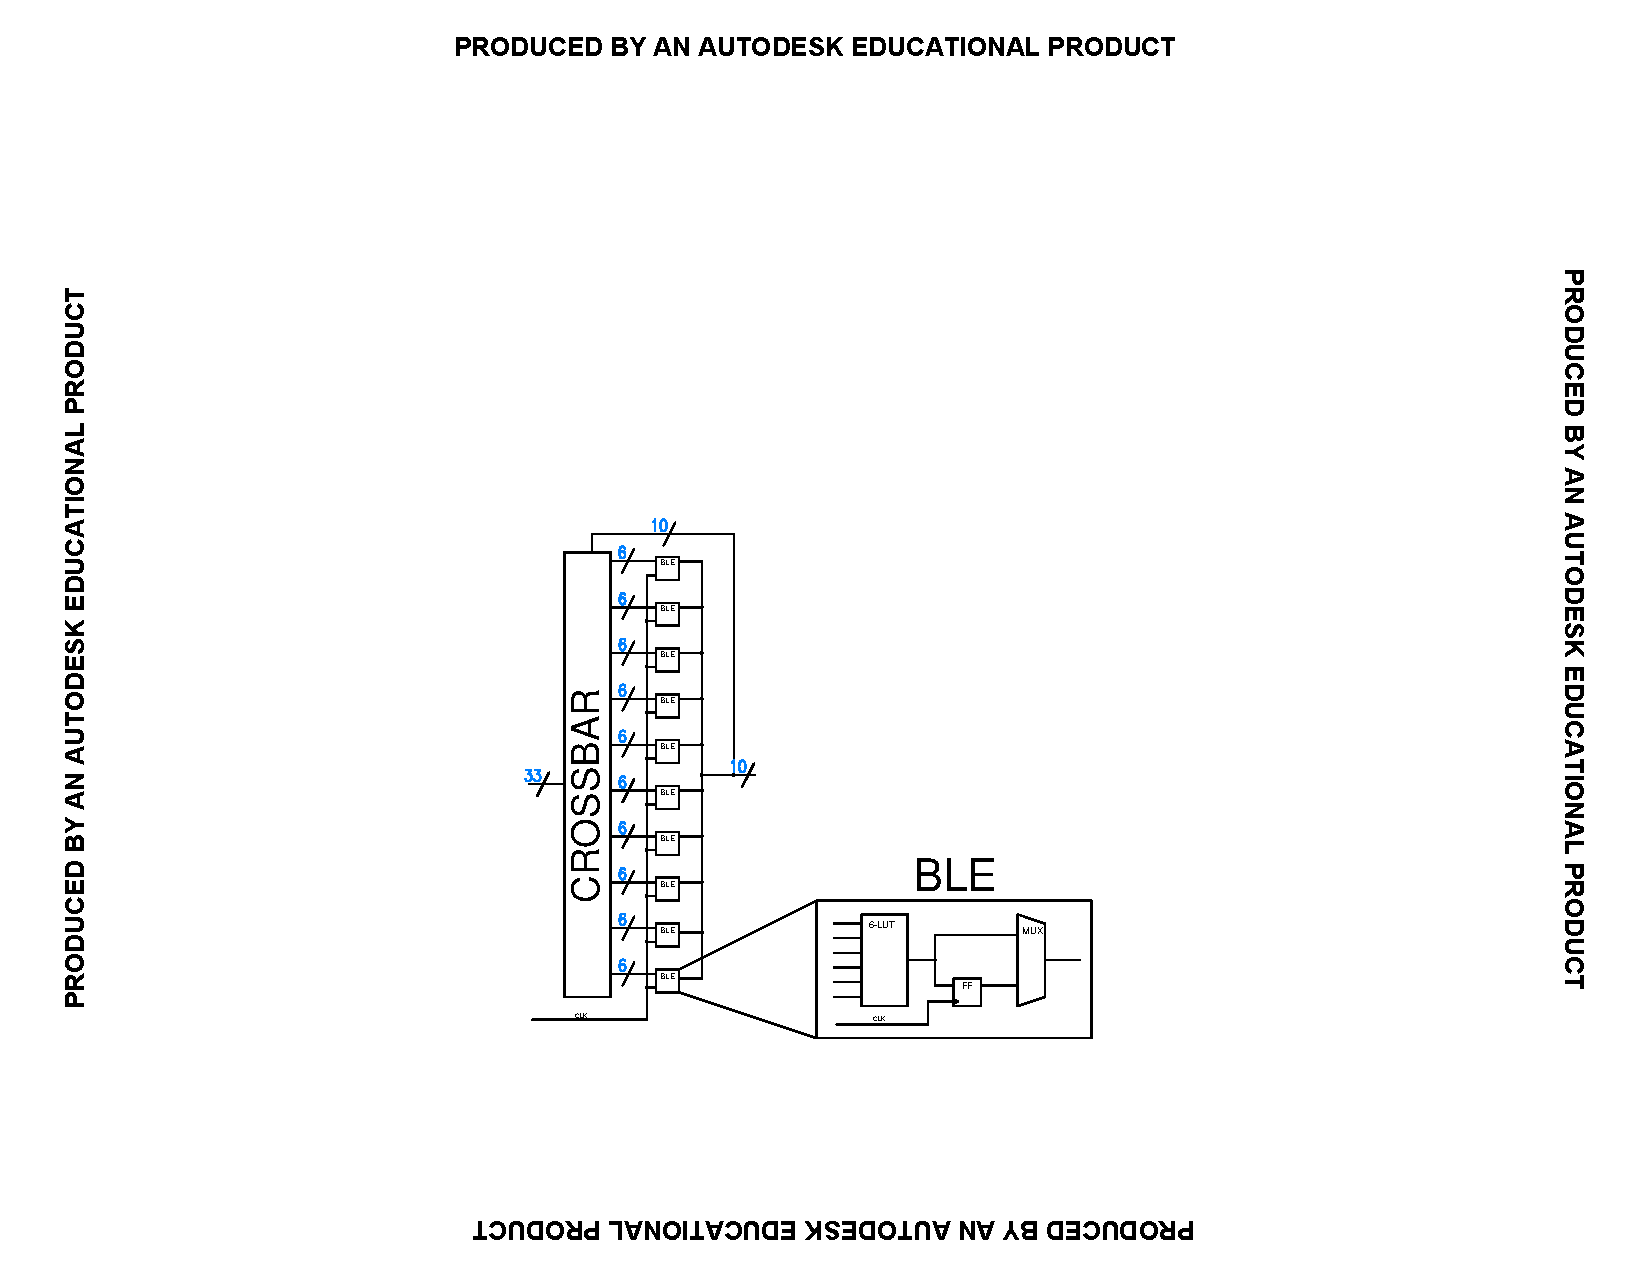
\includegraphics[clip,trim=5cm 4cm 5cm 8cm]{images/CLB.pdf}
    \caption{CLB Architecture}
    \label{Arch}
\end{figure}
VPR allows us to specify a custom architecture for it to run against in an XML format, which for those interested is well documented at \fixme{TODO: reference}. As knowledge of the format is rather tangential to the goal of this thesis we will only be discussing the architecture we used, and not the specifics of the format.

The format is fairly similar to the Virtex 5, consisting of a grid of \acp{CLB} each consisting of ten fully interconnected \acp{BLE}, and each \ac{BLE} having a latch and 6-\ac{LUT}.
Each \ac{BLE} has 6 inputs and 1 output and each \ac{CLB} has 33 inputs and 10 outputs.
Routing resources consist of a configurable number of unidirectional length 4 tracks with \ac{Wilton} switches.

\ctable[
    botcap,
    caption = Architecture Elements,
    label = Arch
]{llll}{
    \tnote{Maximum time.}
}{
    Component & Number & Delay (s) & Notes\NN
    Flip Flop & 1 per BLE & 3.221e-11 & Shown as FF on Diagram\NN
    6-LUT & 1 per BLE & 2.690e-10 & \NN
    MUX & 1 per BLE & 0 * \NN
    BLE & 10 per CLB & 0 &\NN
    Crossbar & 1 per CLB & 8.044e-11\tmark&\NN
    CLB & Autosized by VPR & 0 & \LL
}

\section{Methodology}
To start with, we wanted to collect rough estimates on the impact of partitioning a circuit, to allow us to evaluate whether it's worthwhile proceeding, and to develop the rough estimates needed for our partitioning algorithm. To that end we first created a simple Python script to take an arbitrary input circuit, triplicate it, and insert arbitrary voter logic. These triplicated circuits were then placed and routed by \ac{VPR}, as were the original benchmarks, and the results compared.

\ac{VPR} is used with our architecture file \fixme{TODO: reference} and the command line options 
\begin{lstlisting}
VPR architecture.xml circuit.blif --full_stats[ --route_chan_width x]
\end{lstlisting} where x is the width of the routing channels.
If --route\_chan\_width is excluded then \ac{VPR} determines the minimum channel width needed to successfully route the circuit \fixme{TODO: reference}. We then place and route our benchmark circuits and our partitioned circuits. \ac{VPR} itself then reports the area usage, critical path time, and other statistics we analysed. \ac{VPR} does not unfortunately report the number of pipeline steps, however our partitioner will as it needs to calculate the number of steps for its time estimation function.
\fixme{TODO: List of defaults for VPR parameters}

The place and route process has a random factor to it, due to the methods used (simulated annealing for placement \fixme{TODO: reference} and \fixme{TODO: what does it use to route?}), however generated results are usually within \fixme{TODO: How close and reference} of each other, so to save time the placement and routing process is only run once per circuit (depending on circuit and parameters, a circuit may take in excess of several hours to place and route for some extreme cases.
\section{Results}
The results listed in this section highlight information of interest in a few key circuits, rather than including page after page of tables. Any aggregate statistics (e.g. median) are calculated on the entire result set, not just the results included. No collected results were considered to be outliers or excluded.
These tables list scale factors, that is, $\frac{TMR}{Non-TMR}$.
\begin{table}
    \begin{adjustwidth}{-1cm}{-1.1cm}
        \begin{tabularx}{1.1\textwidth}{XXXXXXXXXXXXXXXXXXXXXXXXXX}
           \toprule
            Name & Input & Output & .latch & .names & FPGA Width & Channel Width & Av. Wire Segments & Used Area & Critical Path & VPR Time\\
          \midrule
            Auto Width & 1 & 1 & 3 & 3.01 & 1.69 & 1.19       & 1.06 & 3.01 & 1.08 & 4.05\\
            200 Width         & 1 & 1 & 3 & 3.01 & 1.69 & 1                & 1.10 & 3.01 & 1.17 & 3.85\\
            60 Width           & 1 & 1 & 3 & 3.01 & 1.69 & 1                & 1.13 & 3.02 & 1.16 & 4.44\\
          \bottomrule
        \end{tabularx}
        \caption{Median Scale Factors for specified channel widths}
        \label{medianRes}
    \end{adjustwidth}
\end{table}

\begin{table}
    \begin{adjustwidth}{-1cm}{-1.1cm}
        \begin{tabularx}{1.1\textwidth}{XXXXXXXXXXXXXXXXXXXXXXXXXX}
           \toprule
            Name & Input & Output & .latch & .names & FPGA Area (width in CLBs) & Av. Wire Segments & Used Logic Block Area & Critical Path & VPR Time\\
            \midrule
pdc 200 width & 1 & 1 & 0 & 3.00 & 1.76 & 1.04 & 3.01 & 1.33 & 4.25\\
          \bottomrule
        \end{tabularx}
        \caption{Scale factors for circuit with maximum critical path slowdown}
        \label{maxRes}
    \end{adjustwidth}
\end{table}
\section{Discussion}
Our simple voter circuit consists of one 3-\ac{LUT} per output. Therefore we expect the number of logic elements (latches and combinational logic) to be exactly three times larger, with an additional 3-\ac{LUT} per original circuit output. As shown in table \ref{medianRes} our triplicated circuits are just slightly over three times as large. Circuit area should be roughly tripled as well, which again, matches, with the width increasing by $1.69 \approx \sqrt{3}$ and the used area increasing by just over triple. The partitioned circuits require slightly larger channels, in order to route the extra wires needed, and the additional elements and wires lead to slightly more segments per wire, and a slightly long critical path. Of note is that the time to place and route the partitioned circuits was much higher, taking around four times longer.

\ref{maxRes} is our worst case slowdown, with a critical path of 33\% longer.



\chapter{Partitioning Algorithm}
\section{Overview}
In this section we discuss the partitioning algorithm, including how we're implementing it, progress, and the reasoning behind design choices made.
\section{Design}
Partitioning in action
•Start with inputs.
Partitioning wavefront
•TMR-ify node-set.
•Repeat process until all nodes are TMR’d.
•Add nodes in a breadth first manner.
•Continue until area, frequency or critical path exceeds threshold.
Max recovery time
Estimated recovery time
Area
Critical Path
Frequency
1.00E-08
1.00E-09
20
1
100MHz
5.00E-30
2
64MHz
2.00E-08
40
50MHz

To do this, need a way of efficiently calculating area, frequency and pipeline length for a set of nodes.
•Pipeline length is trivial, the other two not so much.
•No way to tell until design is routed, which takes too long, therefore we need some way of estimating.
•Also, to effectively traverse, need circuit as a graph. VHDL/Verilog too high level, needs to happen post-synthesis, somewhere in CAD flow.
----------------------------------------------------------------------------


Given a \ac{DFG} our goal is to traverse the \ac{DFG} and partition it, such that every node is in exactly one partition, and the recovery time for each partition is less than our limit.
To do so we traverse the \ac{DFG} in a breadth first manner, keeping track of the critical path length, area, and maximum frequency, extending our partition area as we do so, until our recovery time constraint would be violated. At that point we triplicate our partition, insert our additional voting logic, and then repeat for a new partition, until all nodes have been partitioned.  While doing so we must make sure that no loops exist within a partition, and that all values are voted on before being reused. This is accomplished by making sure that each node is only added once, and when inserting the voting logic that all outputs are voted on before being used as inputs.
A possible improvement in future is improving the traversal algorithm to be more intelligent than just breadth first, to try and maximise each partition's size, though further work will be needed to determine if such optimisations are effective.
\fixme{TODO: pictures and worked example}

\subsection{Design Choices}
As much as possible, we'd like our partitioner to be easily extensible to multiple architectures. The actual partitioner operates on a \ac{DFG} so can be mostly architecture agnostic, only requiring the estimation functions to be architecture aware.
We already have python scripts written to create our benchmark circuits which are able to manipulate \ac{BLIF} files, so we opted for a toolchain incorporating them to reduce development time before we have a working implementation. Specifically, our partitioner operates on \ac{BLIF} files, then just generates separate \ac{BLIF} files for each partition, leaving our Python scripts to perform the actual triplication, insertion of additional elements, and stitching them together. Given time we would like to combine the functionality into one program, however this is a lower priority than developing a working implementation.

Other design choices include deciding on \ac{VPR}, discussed earlier in \fixme{TODO: reference}, namely that its free and open source nature made it amenable to modification, and possible to examine how every step operates, rather than being a black box using some proprietary file format and algorithm, and how we traverse our \ac{DFG}. A depth first traversal would tend to generate long narrow pipelines within each partition, thus increasing critical path length, whereas a breadth first traversal would lend itself to shorter critical paths for the same number of nodes. A possible future improvement is implementing a more advanced traversal algorithm, for example A* with an appropriate heuristic could allow for a higher element density per partition.

Additionally, we were faced with a choice of when in the \ac{CAD} design process (outlined in \fixme{TODO: reference}) to partition. The closer to the end of the process the more control we have, and the better our ability to estimate area and timing, however the harder it is to partition. As we are inserting new elements we want to partition before packing/placement to allow \ac{VPR} to pack and place our inserted elements.

\subsubsection{Choice of Language}
We're using a combination of languages, mainly Python and C++. Language choice primarily came down to preference regarding familiarity personal taste, however a few other considerations were kept in mind.
For \ac{BLIF} joining and insertion of the voting logic Python was used. \ac{BLIF} files are plain text and the text parsing to join and insert is computationally simple, so the primary concern was short development time while still being readable and maintainable.
For the actual partitioner C++ was chosen for a few reasons. Firstly, it was expected that the area and time estimations could be quite computationally expensive, so a lower level compiled language was chosen for performance reasons \fixme{Reference?}. Secondly, \ac{VPR} is written in C, so using C or C++ allowed for easy code reuse, or merging the partitioner and \ac{VPR}. Our reason for choosing C++ over C was that we preferred an object oriented language, as we felt it would be easier to maintain, and would better lend itself to our goal of extensibility, as well as its libraries (e.g. \ac{STL}) making our implementation much easier).

\section{Input file format}
A detailed description of the \ac{BLIF} file format can be found at \fixme{TODO: reference}, however an overview of the format and features used is included below.
\begin{lstlisting}[caption=Sample BLIF file, label=SampleBlif]
.model voter
.inputs a b c
.outputs out
.names a b c out
11- 1
1-1 1
-11 1
.end
\end{lstlisting}
A \ac{BLIF} file is a plain text file which simply lists all the elements of a circuit, and their inputs and outputs. \ac{VPR} (and hence our partitioner) only supports a subset of the \ac{BLIF} file format, detailed in table \fixme{TODO: reference, and insert table}.

A \ac{BLIF} file consists of a module declaration (.module), followed by a list of all input elements (.inputs in1 in2 ...), then a list of all outputs (.outputs out1 out2 ...), then a list of clocks (.clocks clk1 clk2 ...), then a list of all the circuit elements (.latch (latch) and .names (combinational logic)), and finally an optional .end.
\ac{VPR} only supports flat \ac{BLIF} files, so only one module declaration is allowed per \ac{BLIF} file. \ac{SIS} or \ac{ABC} \fixme{TODO: Check that ABC can flatten?} can be used to flatten \ac{BLIF} files for use by \ac{VPR}.

\section{Implementation}
Our implementation is still incomplete, and so is both liable to change, and doesn't currently match our intended design. Most notably, we partition first, then triplicate, then join into one file, rather than triplicating as we partition. A simple pseudocode description is included in \ref{Pseudocode} (omitting code to read and write \ac{BLIF} files), and is discussed below.

Reading in the \ac{BLIF} file is a relatively simple process as subcircuits aren't supported. We make one pass through the input file, reading in the list of inputs, outputs and clocks, and creating a node for each element. We then iterate through the set of nodes building a list of signals, with each signal storing its sources and sinks.

\begin{lstlisting}[caption=Simplified Pseudocode,label=Pseudocode]
Model = new BlifModel(file)
Queue = new Queue()
for each(Signal in Model->Inputs)
    Queue.Push(Signal->Sinks)
Partition = new Partition()

while(Queue.Size > 0)
    Node = Queue.Pop()
    if(AlreadyUsed(Node))
        continue
    if(EstimatedRecoveryTime > MAXIMUM_FAULT_RECOVERY_TIME)
        WritePartitionToFile(FileName, Partition)
        Partition = new Partition()
    Partition.Add(Node)
    for each(Signal in Node->Signals)
        Queue.Push(Signal->Sinks)
        
CombinePartitions()
\end{lstlisting}

As mentioned in section \fixme{Reference}, our input file format is a text file listing all the nodes. We read the file into memory, store it as a \ac{DFG}, with all nodes and signals additionally stored in a hashmap to allow for quick random access. Each node contains a list of all connected signals, and each signal contains a list of all its sources and sinks making the \ac{DFG} quite easy to traverse. Additionally we store a status for each node indicating whether it's part of the current partition, a previous partition, or new, allowing us to detect feedback loops and avoid adding nodes multiple times.
We then traverse the \ac{DFG} in a breadth first matter while keeping running track of an estimate of the current partition's area and timing information. Once adding a new node would exceed our constraints we write the set of contained nodes to an output \ac{BLIF} file, and proceed partitioning the rest. Eventually we have one \ac{BLIF} file for each partition. We then pass these to a set of existing Python scripts, written for initial benchmarking purposes and described in section \fixme{TODO: section} which triplicates each partition and inserts voting logic, then connects each partition back up in a hierarchical \ac{BLIF} file. This file is then passed to \ac{SIS} \fixme{TODO: reference/explain} to be flattened, at which point the partitioned circuit is ready for \ac{VPR}.


\section{Estimating restrictions}
As mentioned earlier, in order to partition our circuit we need a method of calculating the partition's (including voter logic) recovery time, which is based on circuit area (affects time to reconfigure), critical path length (affects time to resynchronise), and frequency (affects time to detect error and resynchronise). Calculating critical path length is relatively easy for our supported input format, as it's just the number of latches on the critical path, which is easily calculated while we traverse the \ac{DFG}.
Area and timing information are more difficult as they rely on the placement and routing of the circuit. Placing and routing each partial partition every step as we traverse is not computationally feasible in a reasonable amount of time, as placement and routing are relatively slow processes and one of our goals is for our partitioning stage to be approximately as fast as the other stages. Therefore, we need a way of estimating them. To do so we've collected preliminary benchmark information for a number of test circuits and analysed them for patterns allowing us to accurately guess area and timing from a given circuit without placing and routing.

\subsection{Results for Time and Area Estimation}
\fixme{TODO: All the graphs and tables of our estimation stuff}
\begin{figure}
    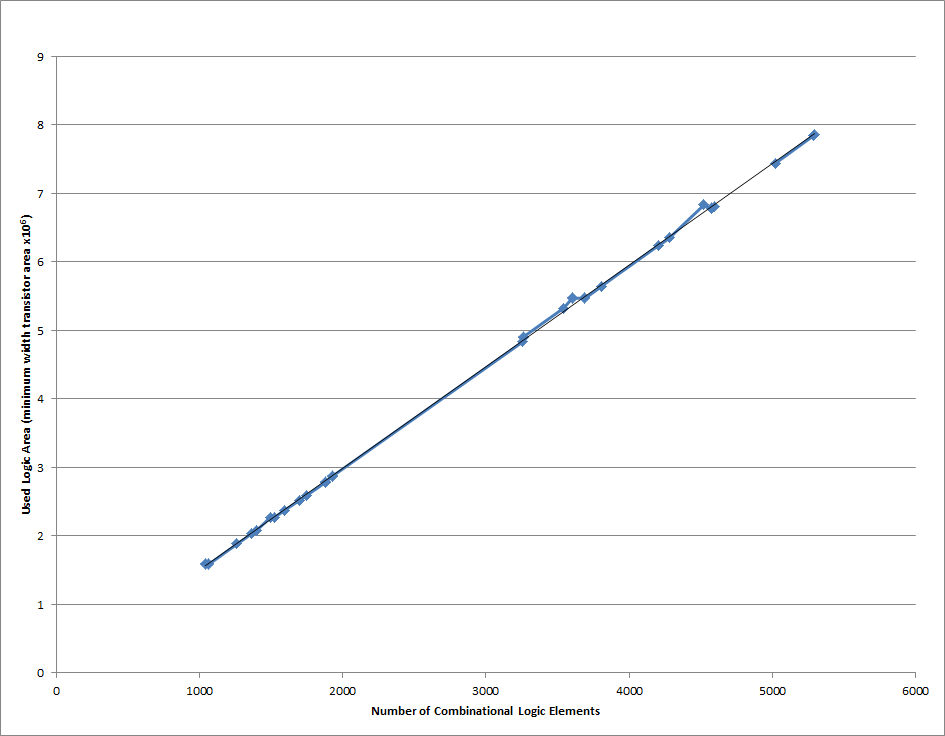
\includegraphics[width=\textwidth]{images/area-v-elements.png}
    \caption{Circuit Area compared to number of Logic Elements}
    \label{AreaVElements}
\end{figure}
\subsection{Discussion of Time and Area Estimation}
As is shown in the results \fixme{TODO: table/graph reference} the area usage is can be accurately estimated, as there is a clear relationship between the number of nodes and the area usage. The architecture we're using \fixme{TODO: reference to where we describe it and what it has} has one latch and one \ac{LUT} per \ac{BLE}, so for our supported logic elements the number of \acp{BLE} used close to linear in $max(num_{latch}, num_{names})$. \ac{VPR}'s packer can be either timing or area driven, currently we are using default settings (mostly area driven) giving us the linear relationship shown in Figure \ref{AreaVElements}. After we have a basic partitioning algorithm an area of further investigation is the impact of changing \ac{VPR}'s settings on the benchmark results, and the accuracy of our estimation functions.

Timing information, on the other hand, is harder to estimate, with no obvious pattern. Generally the maximum frequency is within 10\% slower, though for some cases it goes down to 30\% slower. Conversely, for a few rare cases the partitioned version is actually faster. Initially we will do a rough place and (optionally) route of the original circuit to determine a base time, then multiply it by an experimentally determined slowdown factor to obtain an estimate for the frequency. Initially we're using a slowdown factor of 2 (so half speed after partitioning) which easily encompasses all test circuits we've tried. We can then modify this factor by hand to examine if the impact of it on the final partition's performance warrants improving our estimation function.


\section{Progress}
Still in progress, hopefully nearly finished with first cut.
Done:
\begin{itemize}
    \item Can read a \ac{BLIF} file into a \ac{DFG}.
    \item Can traverse a circuit represented as a \ac{DFG}
    \item Have basic area and timing estimation functions.
    \item Can triplicate an arbitrary circuit (in a single \ac{BLIF} file) and insert arbitrary voter logic (stored in another \ac{BLIF} file).
    \item Initial benchmarks.
\end{itemize}
To Do (above the line is minimum, below the line are nice extras we will be aiming for):
\begin{itemize}
    \item Write \ac{DFG} to \ac{BLIF}.
    \item Incorporate Python scripts into partitioning toolchain.
    \item Benchmark initial partitioning algorithm.
    \item Improve partitioner benchmarks.
    \item ------------------------------------
    \item Investigate the effect of changing \ac{VPR}'s default parameters upon our results.
    \item Combine functionality of Python scripts and C++ partitioner into one program.
    \item Incorporate that single program into \ac{VTR}'s design flow, likely as part of \ac{VPR}.
\end{itemize}
\chapter{What next}
\section{What is still to be done}
•Using very basic and arbitrary estimation functions for area and timing, implement partitioning.
•Improve estimates.
\section{Schedule}
Tuesday Week 12: This report due.

Rest of Week 12 to early Week 13: Catching up on other work/subjects.

Stuvac/Exam period: First cut of partitioning algorithm, start collecting benchmarks.

Holidays: Collect more benchmarks, start analyzing results, play around with \ac{VPR} settings.

Holidays: Data mine results for relationships to improve estimation functions.

Next Year: Keep tweaking estimation functions to try and improve performance, up until Demo and Thesis B due. Extract good/interesting results to discuss further.

Demo.

Thesis B.
\chapter{Conclusion}
All on track, difficult parts will be timing estimates, algorithm may be somewhat restricted in real world applications to problems i.e. better suited for benchmarking the effects of TMR upon a circuit, then actually automatically partitioning a circuit.

\appendix{Glossary}
Quick explanations of what things are (BLE, CLB, DFG, Wilton, etc)

\bibliographystyle{apalike}
\bibliography{../Bibtex/thesis}

\end{document}

%TODO: critical path length -> pipeline steps.
%consistent frequency vs critical path length/latency

%NOTES/QUESTIONS:
%Talk about other FPGA technologies? SRAM, EPROM, EEPROM, FLASH, FUSE, ANTIFUSE, etc.
